\documentclass[11pt,a4paper]{article}

\usepackage[utf8]{inputenc}
\usepackage[T1]{fontenc}
\usepackage[brazil]{babel}
\usepackage{lmodern}
\usepackage[a4paper, margin=2.5cm]{geometry}
\usepackage{amsmath}
\usepackage{booktabs}
\usepackage{float}
\usepackage{caption}
\usepackage{fancyhdr}
\usepackage{graphicx}
\usepackage{pgfplots}
\pgfplotsset{compat=1.18}
\usepackage[hidelinks]{hyperref}

\captionsetup{font=small, labelsep=endash}
\setlength{\parindent}{1.25cm}
\setlength{\parskip}{4pt}

\pagestyle{fancy}
\fancyhf{}
\fancyhead[C]{\small Projeto Integrador -- Engenharia de Computação, 2º sem. 2026 -- IFSP Guarulhos}
\fancyfoot[C]{\thepage}
\renewcommand{\headrulewidth}{0.4pt}

\begin{document}

\begin{center}
	{\Large\bfseries LUXIF: um luxímetro simples e replicável, com LDR, microcontrolador e bateria}

	\vspace{12pt}

	{\small
	EDUARDO L. MARTINEZ\textsuperscript{1}, EMILY O. ARAUJO\textsuperscript{2},
	HENRIQUE F. DEFAVERE\textsuperscript{3}, RAFAEL SHIGUEMI U. RAMOS\textsuperscript{4},
	VINÍCIUS M. PEREIRA\textsuperscript{5}}
\end{center}

\vspace{4pt}
{\footnotesize
\noindent\textsuperscript{1}Graduando em Engenharia de Computação, IFSP, Câmpus Guarulhos, eduardo.martinez@aluno.ifsp.edu.br;\\
\textsuperscript{2}Graduanda em Engenharia de Computação, IFSP, Câmpus Guarulhos, araujo.emily@aluno.ifsp.edu.br;\\
\textsuperscript{3}Graduando em Engenharia de Computação, IFSP, Câmpus Guarulhos, h.defavere@aluno.ifsp.edu.br;\\
\textsuperscript{4}Graduando em Engenharia de Computação, IFSP, Câmpus Guarulhos, rafael.shiguemi@aluno.ifsp.edu.br;\\
\textsuperscript{5}Graduando em Engenharia de Computação, IFSP, Câmpus Guarulhos, vinicius.pereira2@aluno.ifsp.edu.br}

\vspace{8pt}
\noindent\textbf{Área de conhecimento (Tabela CNPq):} 1.05.00.00-6 Física

\vspace{8pt}
\noindent\textbf{RESUMO:} A medição da intensidade luminosa é uma etapa importante em experimentos de óptica e em aplicações de monitoramento ambiental, mas luxímetros comerciais são caros. Este trabalho apresenta o LUXIF, um projeto que mostra como montar um luxímetro simples e replicável, com microcontrolador e bateria, sem a pretensão de ser um instrumento de precisão. O sensor é um fotoresistor (LDR) de 10~mm, que forma um divisor de tensão com um entre quatro resistores de referência, escolhido automaticamente por um Arduino Uno conforme a leitura do conversor analógico-digital, o que amplia a faixa útil de medição e melhora o aproveitamento da sua resolução. A faixa em uso é indicada por LEDs que compartilham um único resistor, e o valor calculado em lux é exibido em um display OLED. O circuito é alimentado por uma bateria de 9~V ligada ao conector de alimentação da placa. A análise teórica indica que as quatro faixas se sobrepõem e cobrem, juntas, resistências de cerca de 100~$\Omega$ a 4~M$\Omega$, o que corresponde a cerca de 0,003 a 11\,000 lux. Por causa de um projeto de extensão, acrescentou-se uma versão opcional com ESP32, que transmite as leituras por Wi-Fi para uma página web.

\vspace{4pt}
\noindent\textbf{PALAVRAS-CHAVE:} fotoresistor; instrumentação eletrônica; divisor de tensão; iluminância; Arduino; ESP32; sensores.

\section*{INTRODUÇÃO}

A medição da intensidade luminosa é fundamental para a realização de experimentos em óptica, permitindo a análise quantitativa de fenômenos como absorção, transmissão e polarização da luz. A utilização de instrumentos de baixo custo para esse fim contribui para a integração entre conceitos teóricos e aplicações práticas em disciplinas de Física e Eletrônica (HALLIDAY; RESNICK; WALKER, 2016).

Os fotoresistores (LDRs) são amplamente utilizados em sistemas de medição luminosa devido à sua simplicidade e ao fato de apresentarem variação de resistência elétrica em função da intensidade de luz incidente (SCHERZ; MONK, 2013). Entretanto, essa resistência varia em várias ordens de grandeza, de centenas de ohms sob luz forte a milhões de ohms no escuro, o que reduz a sensibilidade das medições quando se utiliza apenas um resistor fixo no circuito de leitura.

Diante desse problema, este trabalho propõe um luxímetro em que o microcontrolador escolhe, entre quatro resistores de referência, aquele mais adequado à luz do momento, de forma semelhante à troca automática de escala de um multímetro. O objetivo não é construir um instrumento de precisão, e sim oferecer uma base simples e replicável, que qualquer pessoa possa montar com componentes baratos, entender e melhorar. Por isso, o projeto publica, junto com este texto, o esquema elétrico, a lista de materiais, o código e um passo a passo de montagem, disponíveis em \url{https://github.com/e-arauj0/LUXIF}. A versão com ESP32, que envia as leituras pela internet, foi acrescentada por causa de um projeto de extensão e é uma parte secundária e opcional: o luxímetro funciona sozinho, apenas com o Arduino.

\section*{MATERIAL E MÉTODOS}

O projeto foi desenvolvido a partir de pesquisa bibliográfica em livros, manuais e folhas de dados dos componentes, seguida da modelagem teórica do circuito. Os componentes utilizados estão listados na Tabela~\ref{tab:componentes}.

\begin{table}[H]
	\centering
	\caption{Componentes do LUXIF.}
	\label{tab:componentes}
	\small
	\begin{tabular}{lcl}
		\toprule
		Componente & Qtd. & Função \\
		\midrule
		Arduino Uno & 1 & Trocar as faixas, ler a tensão e calcular o lux \\
		LDR 10 mm & 1 & Sensor de luz \\
		Resistores de 1, 10, 100 e 470 k$\Omega$ & 1 de cada & Resistores de referência das faixas \\
		LED azul & 4 & Indicar a faixa em uso \\
		Resistor de 1 k$\Omega$ & 1 & Limitar a corrente do LED aceso (compartilhado) \\
		Display OLED 0,96" (SSD1306, I\textsuperscript{2}C) & 1 & Exibir a leitura \\
		Bateria de 9 V e suporte & 1 & Alimentação portátil \\
		Cabo com plugue P4 & 1 & Ligar a bateria ao conector do Arduino \\
		Chave gangorra & 1 & Ligar e desligar o circuito \\
		Placa perfurada e fios & -- & Montagem \\
		ESP32 (extensão, opcional) & 1 & Substituir o Arduino na versão com Wi-Fi \\
		\bottomrule
	\end{tabular}
\end{table}

\subsection*{Circuito de medição}

O LDR é ligado entre o ponto de leitura e o terra (GND). Cada um dos quatro resistores de referência ($R_n$) é ligado entre esse mesmo ponto e uma saída digital própria do Arduino (D2 a D5). Apenas uma saída é colocada em nível alto (5~V) por vez; as outras são configuradas como entrada, ficando em alta impedância, o que na prática desconecta seus resistores do circuito. O resistor ativo e o LDR formam um divisor de tensão, cuja saída é lida pela entrada analógica A0 (SCHERZ; MONK, 2013):

\begin{equation}
	V = 5 \times \frac{R_{LDR}}{R_n + R_{LDR}}
	\label{eq:divisor}
\end{equation}

\noindent em que $V$ é a tensão em A0, em volts; $R_{LDR}$ é a resistência do LDR e $R_n$ a do resistor ativo, ambas em ohms. Como as duas resistências são positivas, $V$ fica sempre entre 0 e 5~V, que é o limite da entrada analógica. Além disso, mesmo com o menor resistor (1~k$\Omega$), a corrente na saída do Arduino não passa de 5~mA, bem abaixo do limite recomendado de 20~mA por pino.

O conversor analógico-digital do Arduino Uno tem 10 bits e usa os mesmos 5~V como referência, devolvendo uma leitura $N$ entre 0 e 1023. Combinando essa relação com a Equação~\ref{eq:divisor}, a resistência do LDR é obtida diretamente da leitura, sem depender do valor exato da alimentação:

\begin{equation}
	R_{LDR} = R_n \times \frac{N}{1023 - N}
	\label{eq:resistencia}
\end{equation}

\subsection*{Faixa automática}

A cada medição, o microcontrolador lê a entrada A0 dez vezes e calcula a média, para reduzir o ruído. Em seguida, compara o resultado com dois limites:

\begin{itemize}
	\item se $N > 920$ (cerca de 4,5~V), o ambiente está escuro demais para a faixa atual e o próximo resistor, maior, é selecionado;
	\item se $N < 100$ (cerca de 0,5~V), o ambiente está claro demais e o resistor anterior, menor, é selecionado;
	\item caso contrário, a leitura está na região útil e o valor em lux é calculado.
\end{itemize}

Após cada troca, o programa aguarda 10~ms para o circuito estabilizar antes da próxima leitura. Se a leitura ultrapassar 920 já na faixa de 470~k$\Omega$, não há resistor maior a tentar, e o display indica que o limite foi excedido. A Tabela~\ref{tab:faixas} mostra a resistência do LDR coberta por cada faixa.

\subsection*{Indicação da faixa}

Os quatro LEDs azuis são ligados, cada um, entre uma saída exclusiva do Arduino (D8 a D11) e um ponto comum, formado pelos quatro catodos, que vai ao terra por um único resistor de 1~k$\Omega$. Um LED é aceso junto com a faixa correspondente. Como o programa acende apenas um deles por vez, um resistor basta para todos. Os LEDs apagados ficam com o ânodo em 0~V e o catodo em cerca de 2~V, uma polarização reversa pequena, abaixo do limite típico de 5~V dos LEDs. Mesmo que todos fossem acesos por engano, a corrente total continuaria limitada pelo resistor.

Dessa forma, os LEDs ficam fora do divisor de tensão: a queda de tensão do LED azul (de 2,5 a 3~V) não reduz a tensão disponível no divisor nem varia com a corrente, e a medição não é afetada. Com o resistor de 1~k$\Omega$, a corrente no LED aceso fica em torno de 2~mA, suficiente para a indicação visual e bem abaixo do limite de 20~mA por pino.

\subsection*{Alimentação e display}

O circuito é alimentado por uma bateria de 9~V ligada, através de uma chave gangorra no fio positivo, ao conector de alimentação do Arduino Uno, cujo regulador interno aceita de 7 a 12~V e fornece os 5~V usados pelo restante do circuito. Como a polaridade do cabo com plugue P4 pode variar, convém conferi-la com um multímetro antes de ligar.

O display OLED é ligado ao barramento I\textsuperscript{2}C do Arduino, nos pinos SDA e SCL (as mesmas linhas de A4 e A5 no Uno R3), e alimentado pelos 5~V e pelo GND da placa. Ao ligar, o display exibe uma animação de abertura de cerca de dois segundos. O esquema completo é apresentado na Figura~\ref{fig:esquema}.

\begin{figure}[htbp]
	\centering
	% Figura gerada a partir de imagens/esquema-eletrico.svg, a mesma usada no site.
	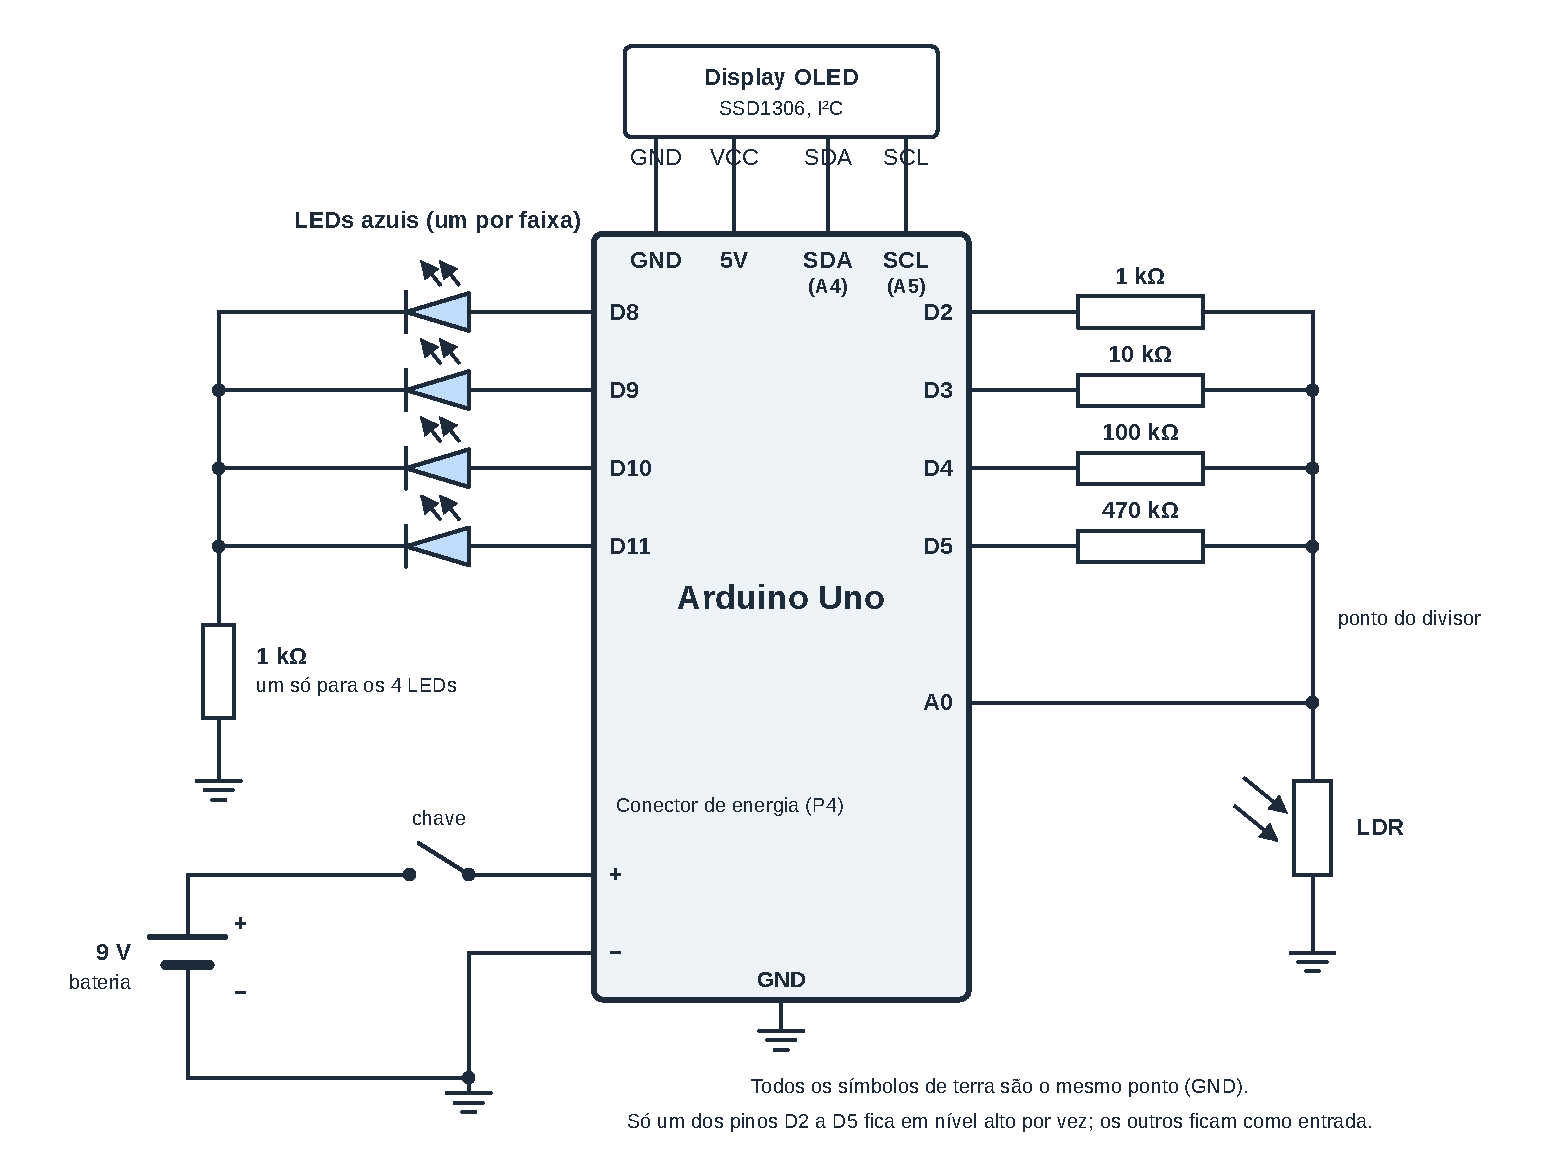
\includegraphics[width=0.95\textwidth]{figuras/esquema-eletrico.pdf}
	\caption{Esquema elétrico do LUXIF.}
	\label{fig:esquema}
\end{figure}

\subsection*{Conversão para lux}

A resistência de um LDR diminui com a iluminância segundo uma lei de potência (SENBA, [s.d.]):

\begin{equation}
	R_{LDR} = A \times L^{-\gamma}
	\label{eq:ldr}
\end{equation}

\noindent em que $L$ é a iluminância, em lux; $A$ é a resistência do LDR em 1~lux; e $\gamma$ indica a inclinação da curva. Foram adotados os valores típicos $A = 75$~k$\Omega$ e $\gamma = 0{,}7$ (Figura~\ref{fig:ldr}). Invertendo a Equação~\ref{eq:ldr}, o microcontrolador calcula a iluminância:

\begin{equation}
	L = \left( \frac{A}{R_{LDR}} \right)^{1/\gamma}
	\label{eq:lux}
\end{equation}

\begin{figure}[htbp]
	\centering
	\begin{tikzpicture}
  \begin{loglogaxis}[
    width=12cm, height=7cm,
    xmin=1, xmax=10000, ymin=100, ymax=100000,
    xlabel={Iluminância (lux)},
    ylabel={Resistência do LDR ($\Omega$)},
    grid=both, minor grid style={gray!15}, major grid style={gray!35},
  ]
    \addplot[domain=1:10000, samples=60, very thick, blue!70!black] {75000*x^(-0.7)};
  \end{loglogaxis}
\end{tikzpicture}

	\caption{Curva teórica da resistência do LDR em função da iluminância, em escala logarítmica.}
	\label{fig:ldr}
\end{figure}

Como dois LDRs do mesmo modelo podem ter curvas diferentes, $A$ e $\gamma$ podem ser ajustados ao sensor em uso. Tomando o logaritmo da Equação~\ref{eq:ldr}, obtém-se $\ln R_{LDR} = \ln A - \gamma \ln L$, uma reta. Com a resistência medida em duas iluminâncias conhecidas, $(L_1, R_1)$ e $(L_2, R_2)$, comparadas a um luxímetro de referência, resultam

\begin{equation}
	\gamma = \frac{\ln(R_1/R_2)}{\ln(L_2/L_1)}
	\qquad\text{e}\qquad
	A = R_1 \times L_1^{\gamma}.
	\label{eq:calibracao}
\end{equation}

\noindent Aplicadas aos pontos da Figura~\ref{fig:ldr} (75~k$\Omega$ em 1~lux e cerca de 120~$\Omega$ em 10\,000~lux), as expressões retornam $\gamma \approx 0{,}70$ e $A = 75$~k$\Omega$, os valores adotados.

\subsection*{Extensão com ESP32}

A versão com ESP32 foi acrescentada por causa de um projeto de extensão. O circuito de medição é o mesmo, com os pinos GPIO 25, 26, 27 e 14 para os resistores de referência, GPIO 16 a 19 para os LEDs e GPIO 34 para a leitura. O conversor analógico-digital do ESP32 tem 12 bits, e a leitura $N$ vai de 0 a 4095, com os limites de troca de faixa em 400 e 3700. As leituras são enviadas como texto JSON, no formato \texttt{\{"lux":523.4,"percentage":100.0,"faixa":1\}}, por dois caminhos: pela internet, com o protocolo MQTT (OASIS, 2014), em que o ESP32 publica as medições em um canal de um servidor e a página web assina esse canal; e pela rede local, com um servidor WebSocket (FETTE; MELNIKOV, 2011) acessado em \texttt{ws://IP/ws}, em que o navegador se conecta diretamente ao ESP32. O servidor WebSocket foi desenvolvido em ESP-IDF e usa o mesmo formato de mensagem, de modo que a mesma página exibe os dados vindos de qualquer um dos firmwares.

\section*{RESULTADOS E DISCUSSÃO}

A Figura~\ref{fig:divisor} apresenta a tensão em A0 em função da resistência do LDR para cada resistor de referência, calculada pela Equação~\ref{eq:divisor}. A região sombreada corresponde à janela de leitura útil, entre 0,5 e 4,5~V. Cada curva é mais inclinada, e portanto mais sensível, quando a resistência do LDR é próxima de $R_n$; longe desse ponto, a curva fica plana e variações de luz quase não alteram a tensão. A troca automática mantém a medição sempre na parte inclinada de alguma das curvas.

\begin{figure}[htbp]
	\centering
	\begin{tikzpicture}
  \begin{semilogxaxis}[
    width=12cm, height=7cm,
    xmin=100, xmax=10000000, ymin=0, ymax=5,
    xlabel={Resistência do LDR ($\Omega$)},
    ylabel={Tensão em A0 (V)},
    grid=both, minor grid style={gray!15}, major grid style={gray!35},
    legend pos=south east, legend cell align=left,
  ]
    \addplot[fill=green!25, fill opacity=0.5, draw=none, forget plot] coordinates {(100,0.49) (10000000,0.49) (10000000,4.5) (100,4.5)} -- cycle;
    \addplot[domain=100:10000000, samples=120, very thick, blue!70!black] {5*x/(1000+x)};
    \addplot[domain=100:10000000, samples=120, very thick, orange!80!black] {5*x/(10000+x)};
    \addplot[domain=100:10000000, samples=120, very thick, green!50!black] {5*x/(100000+x)};
    \addplot[domain=100:10000000, samples=120, very thick, red!70!black] {5*x/(470000+x)};
    \legend{$R_n = 1\,\mathrm{k\Omega}$, $R_n = 10\,\mathrm{k\Omega}$, $R_n = 100\,\mathrm{k\Omega}$, $R_n = 470\,\mathrm{k\Omega}$}
  \end{semilogxaxis}
\end{tikzpicture}

	\caption{Tensão em A0 em função da resistência do LDR para os quatro resistores de referência. A região sombreada é a janela de leitura útil.}
	\label{fig:divisor}
\end{figure}

A Tabela~\ref{tab:faixas} resume a cobertura de cada faixa, obtida aplicando os limites de leitura (100 e 920) à Equação~\ref{eq:resistencia}. Cada faixa cobre resistências de cerca de $R_n/9$ a $9 \times R_n$. Como os resistores vizinhos diferem por um fator de 10 ou menos, as faixas se sobrepõem, o que cria uma histerese natural: quando a luz está perto de um limite, o instrumento não fica alternando entre duas faixas.

\begin{table}[H]
	\centering
	\caption{Cobertura teórica de cada faixa.}
	\label{tab:faixas}
	\small
	\begin{tabular}{cccc}
		\toprule
		Faixa & $R_n$ & $R_{LDR}$ coberta & Iluminância estimada \\
		\midrule
		1 & 1 k$\Omega$ & 108 $\Omega$ a 8,9 k$\Omega$ & 21 a 11\,400 lux \\
		2 & 10 k$\Omega$ & 1,1 k$\Omega$ a 89 k$\Omega$ & 0,8 a 430 lux \\
		3 & 100 k$\Omega$ & 11 k$\Omega$ a 893 k$\Omega$ & 0,03 a 16 lux \\
		4 & 470 k$\Omega$ & 51 k$\Omega$ a 4,2 M$\Omega$ & 0,003 a 1,7 lux \\
		\bottomrule
	\end{tabular}
\end{table}

Juntas, as quatro faixas cobrem, em teoria, de cerca de 0,003 a 11\,000 lux. Esses valores são uma estimativa que depende dos valores de $A$ e $\gamma$ adotados, que são típicos e podem ser ajustados no código para cada sensor, como descrito na subseção \textit{Conversão para lux}. Na prática, as pontas da escala são as menos confiáveis, e o instrumento só pode ser tratado como exato depois de comparado com um luxímetro de referência.

\subsection*{Limitações}

O LUXIF é uma base para aprender a montar um luxímetro, e não um instrumento de precisão. Algumas limitações merecem ser registradas:

\begin{itemize}
	\item \textbf{O sensor.} O LDR não segue exatamente a lei de potência em toda a escala, varia com a temperatura, responde de forma lenta a mudanças de luz e não tem a mesma resposta espectral do olho humano. Fontes de luz com espectros diferentes (sol, LED, fluorescente) podem produzir leituras distintas para a mesma iluminância.
	\item \textbf{A leitura analógica.} O fabricante do microcontrolador recomenda que a fonte do sinal lido pelo conversor tenha impedância de cerca de 10~k$\Omega$ ou menos (MICROCHIP, [s.d.]). Nas faixas de 100~k$\Omega$ e 470~k$\Omega$, com o LDR no escuro, a impedância é muito maior, e a leitura perde exatidão. A média de dez leituras e a espera de 10~ms após cada troca de faixa reduzem o problema, mas não o eliminam.
	\item \textbf{Sem capacitor em A0.} Filtrar o ruído com um capacitor de 100~nF, por exemplo, formaria com resistências de alguns M$\Omega$ um filtro RC de constante de tempo da ordem de 0,4~s, muito maior que a espera de 10~ms, e a leitura ficaria errada logo após cada troca de faixa.
	\item \textbf{O pino de saída.} A saída digital que fornece os 5~V tem resistência interna de algumas dezenas de ohms, que se soma ao resistor de referência e, na faixa de 1~k$\Omega$, já representa alguns por cento do valor.
\end{itemize}

Cada uma dessas limitações é também um ponto de partida para melhorias: trocar o sensor, calibrar o instrumento, filtrar o sinal ou usar um conversor externo.

\section*{CONCLUSÕES}

O presente trabalho apresentou um luxímetro simples e replicável, baseado em um LDR, em quatro resistores de referência e em um Arduino Uno, com a finalidade principal de mostrar como se monta um instrumento desse tipo com microcontrolador e bateria. A análise teórica do divisor de tensão mostrou que a seleção automática entre os resistores mantém a leitura sempre na região de maior sensibilidade, ampliando a faixa dinâmica em comparação com um resistor fixo, em cerca de 0,003 a 11\,000 lux pela estimativa teórica.

Os LEDs indicadores, ligados a saídas próprias e com um resistor único, não interferem na medição, e a alimentação por bateria de 9~V com chave torna o instrumento portátil. As limitações descritas, em especial a falta de calibração, impedem tratá-lo como instrumento de precisão, mas deixam claro por onde melhorá-lo. A versão opcional com ESP32, acrescentada por causa de um projeto de extensão, transmite as leituras por Wi-Fi, pela internet (MQTT) ou pela rede local (WebSocket), para uma página web que as exibe em tempo real.

\section*{CONTRIBUIÇÕES DOS AUTORES}

E.L.M.\textsuperscript{1} contribuiu como principal gerente e organizador do projeto, planejando, coordenando e conduzindo as pesquisas, refinando a base teórica e formulando os objetivos de estudo. H.F.D.\textsuperscript{3} e R.S.U.R.\textsuperscript{4} atuaram como principais investigadores e analistas formais, providenciando os dados e as ferramentas matemáticas, visuais e linguísticas, além de atuarem, de forma secundária, como supervisores e revisores. E.O.A.\textsuperscript{2} atuou como principal editora e revisora de dados, além de validar as informações obtidas e as ferramentas matemáticas utilizadas. V.M.P.\textsuperscript{5} desenvolveu o servidor WebSocket em ESP-IDF para o ESP32, usado na comunicação sem fio das leituras com a página web.

\section*{AGRADECIMENTOS}

Agradecimentos aos professores Dennis Toufen, Maurício Capelas, Hamilton Piva e Wilson Carlos por sua coordenação, ensino, condução e direção, que nos permitiram desenvolver e evoluir tanto este projeto e pesquisa como nossas vidas acadêmicas.

\section*{REFERÊNCIAS}

\begin{flushleft}
\small
ARDUINO. \textbf{Arduino Uno Rev3}: documentação técnica. [S.l.]: Arduino, [s.d.]. Disponível em: \url{https://docs.arduino.cc/hardware/uno-rev3/}.

\vspace{6pt}
HALLIDAY, David; RESNICK, Robert; WALKER, Jearl. \textbf{Fundamentos de Física}: Óptica e Física Moderna. 10. ed. Rio de Janeiro: LTC, 2016.

\vspace{6pt}
FETTE, Ian; MELNIKOV, Alexey. \textbf{RFC 6455}: The WebSocket Protocol. Internet Engineering Task Force, 2011. Disponível em: \url{https://www.rfc-editor.org/rfc/rfc6455}.

\vspace{6pt}
MICROCHIP TECHNOLOGY. \textbf{ATmega328P}: folha de dados (seção do conversor analógico-digital). [S.l.]: Microchip Technology, [s.d.]. Disponível em: \url{https://www.microchip.com/en-us/product/ATmega328P}.

\vspace{6pt}
OASIS. \textbf{MQTT Version 3.1.1}. OASIS Standard, 2014. Disponível em: \url{https://docs.oasis-open.org/mqtt/mqtt/v3.1.1/mqtt-v3.1.1.html}.

\vspace{6pt}
SCHERZ, Paul; MONK, Simon. \textbf{Practical Electronics for Inventors}. 3. ed. New York: McGraw-Hill Education TAB, 2013.

\vspace{6pt}
SENBA OPTOELECTRONICS CO., LTD. \textbf{GL55 Series Photoresistor Datasheet}. Shenzhen: Senba Optoelectronics, [s.d.]. Disponível em: \url{https://www.digikey.com/en/htmldatasheets/production/2014143/0/0/1/gl5528.html}.
\end{flushleft}

\end{document}
